% \chapter{Begin Stream}
\chapter{Verification of the wave equation}
\label{appendix:wave_eq}

\begin{wrapfigure}{r}{.4\textwidth}
    \vspace{-12pt}
    \centering
    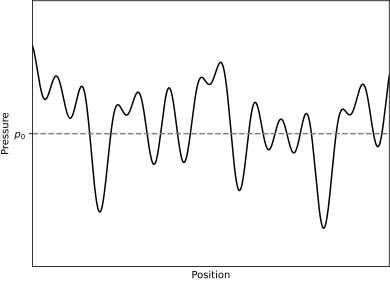
\includegraphics[width=.4\textwidth]{pictures/random_pressure}
    % \captionsetup{justification=centering}
    \vspace{-1.5em}
    \caption{Some function of pressure depending on position that will change with time.}
    \label{fig:pres_pos}
    \vspace{-1.5em}
\end{wrapfigure}

This is an intuitive verification of the one-dimensional acoustic wave equation\footnote{Notation and ideas used in this appendix are adapted from \citeauthor{notation_intuitive} \cite{notation_intuitive}.} (the three-dimensional version is derived in Section \ref{sec:wave_eq}).
To start off with this approach, let us assume that there is no sound.
Then, no vibrations in the air can occur which, in turn, results in equal pressure in the air not varying with position (denoted $p_0$).

However, if there is sound we do get vibrations and therefore some variation of pressure depending on the position you are measuring the sound as can be seen in Figure \ref{fig:pres_pos}.

To gain intuition for what happens over time let us discretize the pressure function and pick only 3 ``adjacent'' points from the function.
This can also be thought of as zooming in on Figure \ref{fig:pres_pos} until you see only 3 points.
An example of this can be seen in Figure \ref{fig:zoom_1}.
We take look at how the pressure of the middle point, $p_2$, changes as a function of its differences with $p_1$ and $p_3$. After rewriting this function we look at the limit and get the partial differential equation named the one-dimensional acoustic wave equation.

So, to begin we start at $t=0$ with Figure \ref{fig:zoom_1}, the three points are denoted $x_1$, $x_2$, and $x_3$ with corresponding pressures $p_1$, $p_2$, and $p_3$, respectively.
We assume that $p_1$ and $p_3$ are fixed and investigate the function $p_2$ describes (note that the values $1$ for $p_1$, $4$ for $p_2$ and $-1$ for $p_3$ are chosen arbitrarily and can be scaled appropriately).
We start with the situation where the air at $x_1$, $x_2$, and $x_3$ has no velocity.
Because there is a high pressure at $x_2$ and lower pressures at $x_1$ and $x_3$, the system wants to ``equalize'' the pressure, and we get a large acceleration of air from $x_2$ towards $x_1$ and $x_3$ (from now on we say that $p_2$ has a large acceleration towards $p_0$, the static pressure), but since the system needs time to ``start up'' the velocity of the individual particles stays small but will increase rapidly. The total change in pressure will thus be little, giving the situation in Figure \ref{fig:zoom_2}.

Now the velocity of the individual particles, i.e. the change in pressure, has started to build up, although the acceleration of $p_2$ towards $p_0$ has started to decrease due to the decreased difference to $p_1$ and $p_3$ (the system does not want to ``equalize'' the pressure as much) thus the velocity of $p_2$ towards $p_0$ will not increase as much as last time. We obtain the situation in Figure \ref{fig:zoom_3}.

The velocity still increases due to a positive acceleration but with each timestep the acceleration decreases. Hence, the velocity will increase less and less, resulting in the situation in Figure \ref{fig:zoom_4}.

At this point we have $p_1=p_2$ meaning that $x_1$ and $x_2$ are in equilibrium, however, $x_2$ and $x_3$ are not. So there will still be a positive acceleration, due to a high velocity, the pressure in $x_2$, $p_2$, shoots past the static pressure $p_0$. At the next timestep we see something like the situation in Figure \ref{fig:zoom_5}.

The velocity starts to decrease because of the difference in pressure at $x_1$ and $x_2$, thus we have negative acceleration. But the velocity is still positive thus we still get a decreasing pressure in $x_2$. Due to the negative acceleration that keeps on increasing as $p_3$ decreases, the velocity will eventually be 0 again. This happens in the situation in Figure \ref{fig:zoom_6}, at $t=7$.

\begin{figure}[h]
    % \vspace{-10pt}
    \begin{tabular}{cccc}
        \subcaptionbox{\centering Situation at $t=0$\label{fig:zoom_1}}{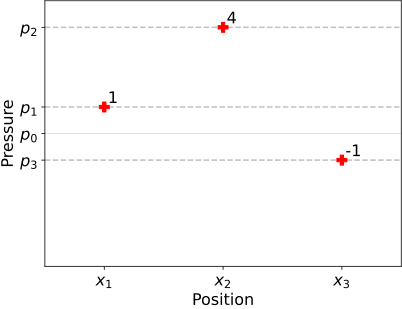
\includegraphics[width=.3\textwidth]{pictures/pressure_zoom_1}} &
        \subcaptionbox{\centering Situation at $t=1$\label{fig:zoom_2}}{\includegraphics[width=.3\textwidth]{pictures/pressure_zoom_2}} &
        \subcaptionbox{\centering Situation at $t=2$\label{fig:zoom_3}}{\includegraphics[width=.3\textwidth]{pictures/pressure_zoom_3}} \\
        \subcaptionbox{\centering Situation at $t=3$\label{fig:zoom_4}}{\includegraphics[width=.3\textwidth]{pictures/pressure_zoom_4}} &
        \subcaptionbox{\centering Situation at $t=4$\label{fig:zoom_5}}{\includegraphics[width=.3\textwidth]{pictures/pressure_zoom_5}} &
        \subcaptionbox{\centering Situation at $t=7$\label{fig:zoom_6}}{\includegraphics[width=.3\textwidth]{pictures/pressure_zoom_6}} &
    \end{tabular}
    \caption{Zoomed in version of Figure \ref{fig:pres_pos}, here $p_1=p(x_1)$, $p_2=p(x_2)$ and $p_3=p(x_3)$. Note that the timesteps can be scaled appropriately.}
\end{figure}

We have gotten a more intuitive feel of how the differences in pressure increase the acceleration of the pressure. To put that thought in formulas, we get that the acceleration of the pressure (its 2nd time derivative) is a function of the sum of differences between $p_1$ and $p_2$ and between $p_2$ and $p_3$, thus after defining some constant $\alpha$ and noting that positive acceleration defined is upwards we get (note that $\Delta$ denotes the spatial difference):
\begin{equation}
    \frac{\partial^2 p}{\partial t^2} = -\alpha (\underbrace{(p_2-p_1)}_{\Delta p_1} + \underbrace{(p_2-p_3)}_{-\Delta p_2}) = \alpha \underbrace{(\Delta p_2 - \Delta p_1)}_{\Delta\Delta p_1} \,.\label{eq:dif_of_dif}
\end{equation}
Thus, $\frac{\partial^2 p}{\partial t^2}$ is a function of the spatial difference of $\Delta p_1$ and $\Delta p_2$, thus it can be denoted by the second spatial difference $\Delta \Delta p_1$.
Now, if we take the limit so that the difference in positions goes to zero ($(x_2-x_1) \to 0$ and $(x_3-x_2) \to 0$ as well). We get that these differences turn into spatial derivates. Then \ref{eq:dif_of_dif} becomes
\begin{equation}
    \frac{\partial^2 p}{\partial t^2} = \alpha \frac{\partial^2 p}{\partial x^2}\,, \nonumber
\end{equation}
which is the one-dimensional acoustic wave equation.
